\section{Generalization and Regularization}
A good model has a low Generalization Error, find the optimal complexity for our model \\

\begin{itemize}
    \item \textcolor{blue}{In-Sample Error} / \textcolor{blue}{Training error} the MSE with known data, minimized during training
    \item \textcolor{blue}{Out-of-sample Error} / \textcolor{blue}{Generalization Error} / \textcolor{blue}{Test Error} the MSE of new data, sagt uns wie gut mein model das gelernte auf neue Daten verallgemeinert, \textcolor{red}{can't be calculated, but estimated}
\end{itemize}

\subsection{Overfitting}
\begin{itemize}
    \item A model that perfectly fits the data does not have to be perfect
    \item In-Sample Error was minimized (MSE = 0)
    \item Overfitting happens if the MSE of Training Error is small thanks to a complex model but the Generalization Error is large (Good with training data, bad with testing data)
\end{itemize}
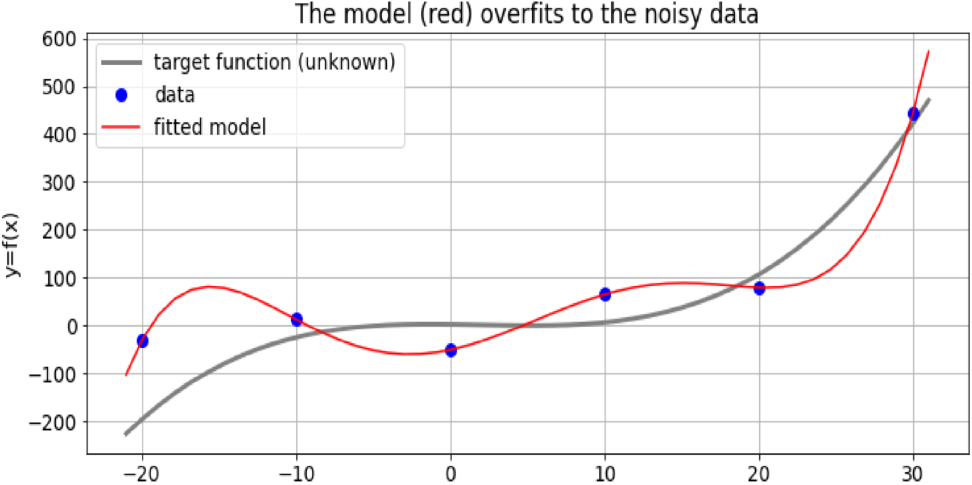
\includegraphics[width=0.9\linewidth]{overfitting.png}

\subsection{Underfitting}
\begin{itemize}
    \item Using a too simple model
    \item In-Sample Error is large
    \item Generalization Error is large
\end{itemize}

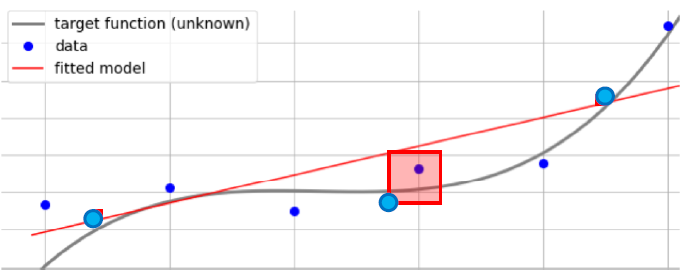
\includegraphics[width=0.9\linewidth]{underfitting.png}

\subsection{Training-Set, Test-Set, Model Evaluation}
\begin{itemize}
    \item Split the data into 2 sets
    \begin{itemize}
        \item Training-Set (~80\% of data)
        \item Test-Set (~20\% of data)
    \end{itemize}
\end{itemize}
\vspace{10pt}
\textbf{Training}
\begin{itemize}
    \item Fit the model to the training set
    \item This minimizes the in-sample error
\end{itemize}
\vspace{10pt}
\textbf{Evaluating}
\begin{itemize}
    \item Using the Test-Set
    \item Produces the \textcolor{blue}{Test-Error}
    \item This is an estimate of the Generalization Error
\end{itemize}

\subsection{Bias-Variance Trade-off}

\textbf{High Bias}
\begin{itemize}
    \item A too simple model for the given data
\end{itemize}
\vspace{10pt}
\textbf{Low Variance}
\begin{itemize}
    \item The model is relatively stable
    \item Very similar model if trained with new data
\end{itemize}
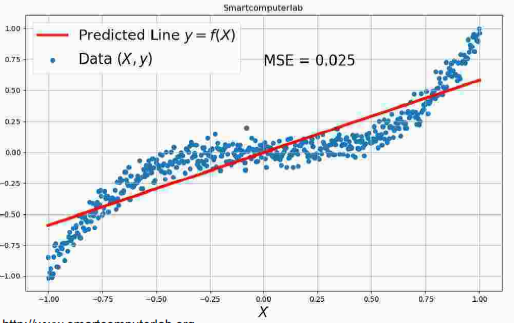
\includegraphics[width=0.6\linewidth]{bias_variance.png}\\

\textbf{Low Bias}
\begin{itemize}
    \item A more complex model can better explain the data
    \item A lot of free parameters
\end{itemize}
\vspace{10pt}
\textbf{High Variance}
\begin{itemize}
    \item Given a new datapoint, the MSE can be very large
    \item For a different set with more datapoints, the model may be very different
\end{itemize}
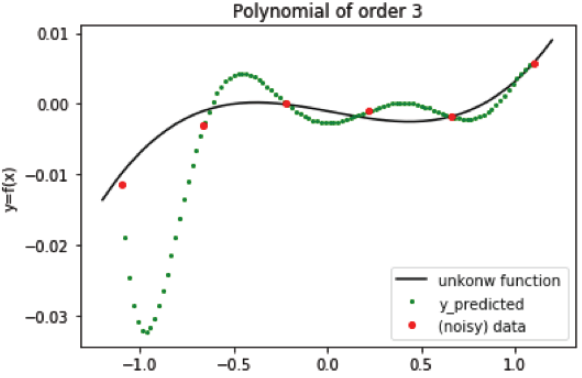
\includegraphics[width=0.6\linewidth]{bias_variance2.png}

\subsubsection{Trade-off}
\begin{itemize}
    \item Higher bias implies lower variance
    \item Lower bias implies higher variance
    \item In practice, \textcolor{blue}{all we want is low variance}
    \item The model can only be as complex as the data permits
    \item You have to find an optimal balance between bias and variance
\end{itemize}
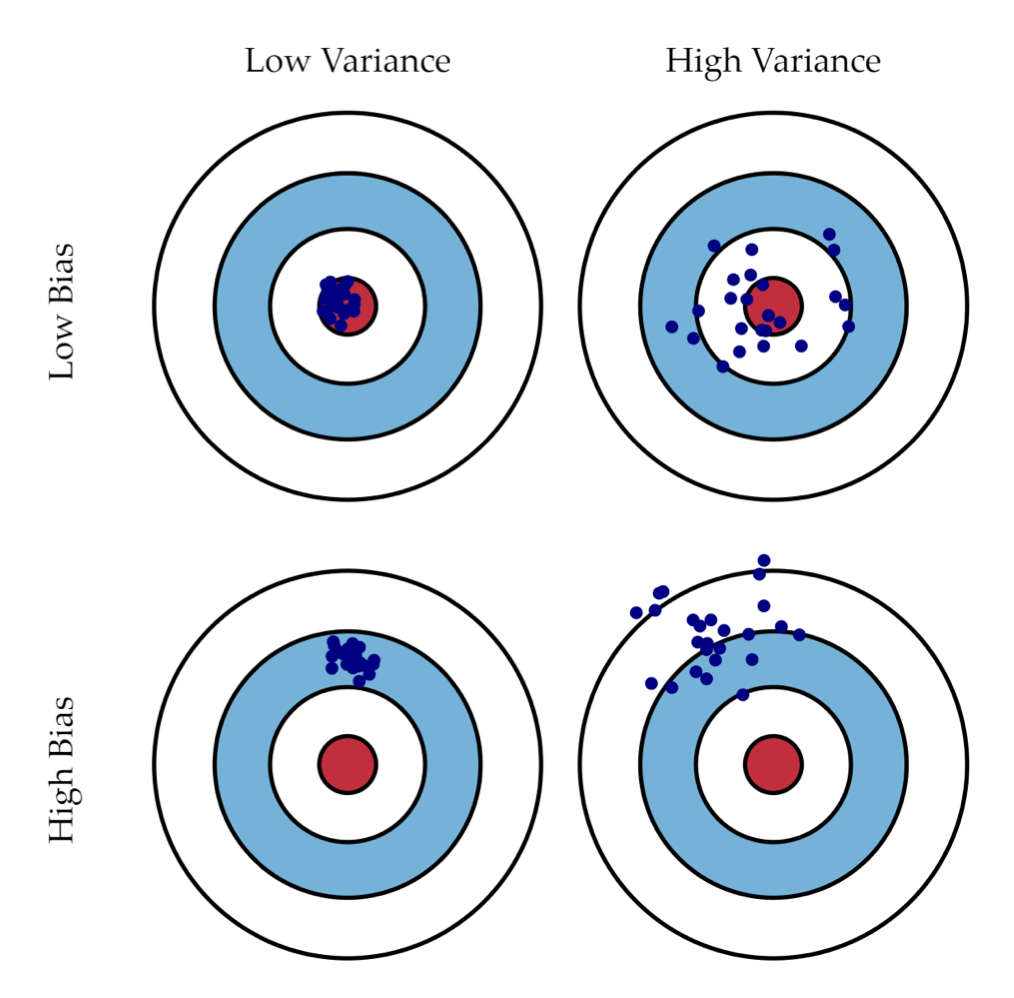
\includegraphics[width=0.8\linewidth]{bias-variance-tradeoff.png}

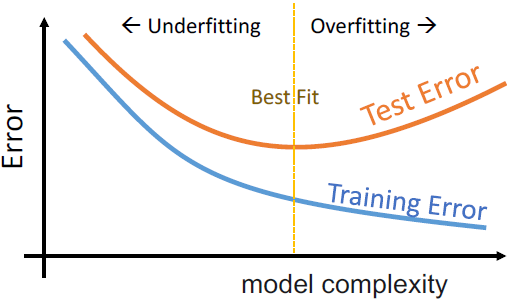
\includegraphics[width=0.6\linewidth]{tradeoff.png}

\subsection{Regularization}
Wird verwendet um \textcolor{blue}{Best Fit} spot zu finden und damit Komplexität zu kontrollieren \\

\textbf{Measuring}

Technique to measure the model complexity
\begin{itemize}
    \item L1 - Norm $\displaystyle\sum_{j = 1}^{p} |\beta_j|$
    \item L2 - Norm $\displaystyle\sum_{j = 1}^{p}\beta_j^2$
\end{itemize}
\vspace{10pt}
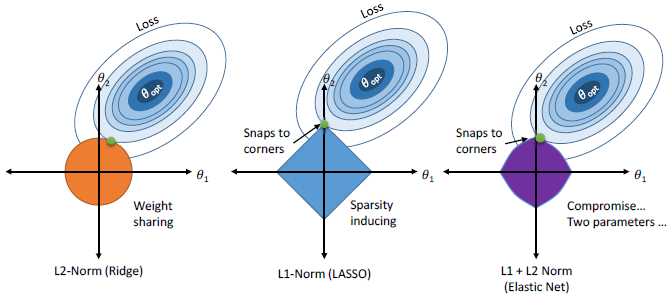
\includegraphics[width=1\linewidth]{regularization.png} \\

\textbf{Controlling}

$\lambda = 0$ implies no regularization

Technique to control the model complexity
\begin{itemize}
    \item Add a penalty term to the Loss (optimization problem)
    \item More complex models get a higher penalty
    \item Add a constrain to the optimization process
\end{itemize}
\vspace{10pt}
Regularization Loss $=$ MSE $+ \lambda *$ model-complexity

\begin{center}
    $\displaystyle\sum_{i = 1}^{n} (y_i - \displaystyle\sum_{j = 1}^{p} x_{ij}\beta_j)^2 + \lambda \displaystyle\sum_{j = 1}^{p}\beta_j^2$
\end{center}
